\chapter{Method}
\label{chap:desarrollo}
\vspace{0.5cm}

%%%%%%%%%%%%%%%%%%%%%%%%%%%%%%%%%%%%%%%%%%%%%%%%%%%%%%%%%%%%%%%%%%%%%%%%%%%%%%%%
% Objetivo: Exponer las partes relevantes de la implementación                 %
%%%%%%%%%%%%%%%%%%%%%%%%%%%%%%%%%%%%%%%%%%%%%%%%%%%%%%%%%%%%%%%%%%%%%%%%%%%%%%%%

\section{Approach}
\label{sec:metodology}

The architecture of \texttt{haspie} (See Figure \ref{fig:arquitectura_final}) is a simple pipeline wirtten in Python with a single execution path. This pipeline calls each submodule passing the correct parameters and then retrieves and parses the output generated by each step of the tool.

\begin{figure}[h]
	\centering
	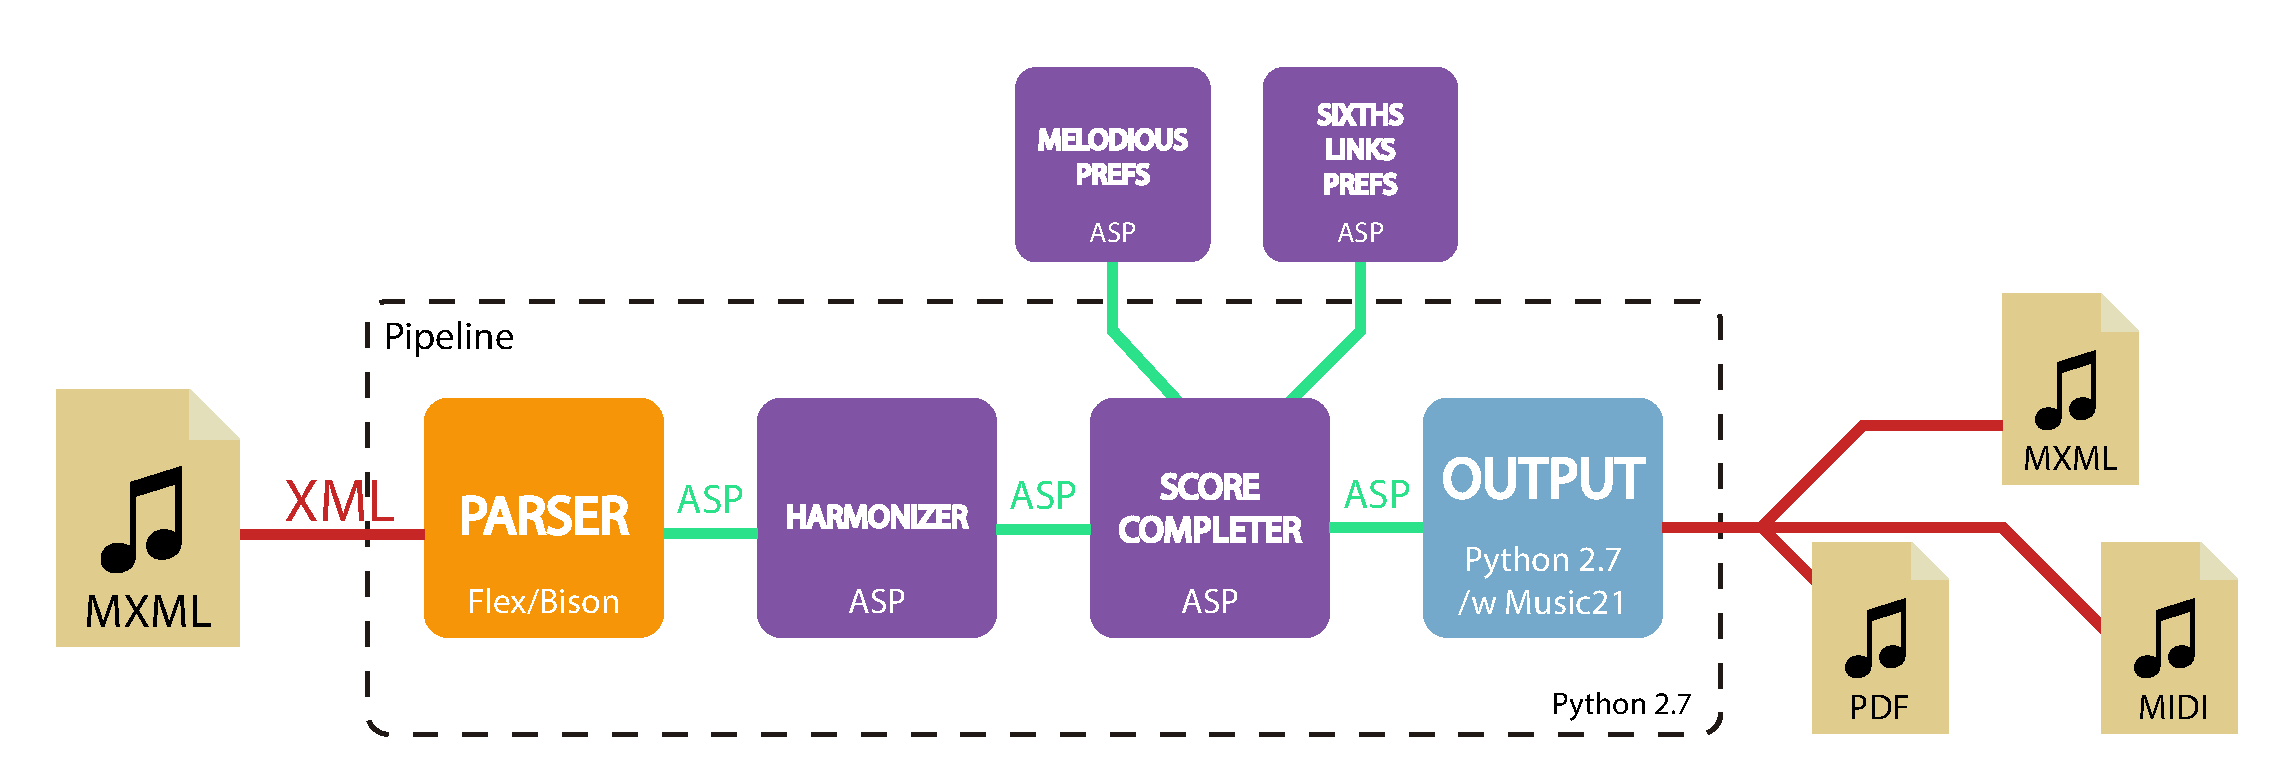
\includegraphics[width=0.8\linewidth]{imagenes/arquitectura_final.pdf}
	\caption{Haspie's Architecture}
	\label{fig:arquitectura_final}
\end{figure}

\subsection{Input}
The tool takes a single MusicXML file as input that is passed to the first stage of the pipeline: a parser written in C along with the Flex and Bison libraries. This module transforms the MusicXML tag information to Answer Set Programming logic facts. This parser does not only parse the musical figures but also performs many other tasks such as:

\begin{itemize}
 	\item Subdividing the figures to standardize the rhythmic patterns.
 	\item Creating additional logic facts to retrieve the original rhythm structures after the score processing.
 	\item Identifying the different measure types.
 	\item Interpreting the instrument names to determine their most common pitch ranges.
 	\item Infer the tonality of the score by parsing it's key.
 	\item Parsing some of the score metadata, such as the piece name or the composer.
\end{itemize}

After the parsing step, all of this extracted data is saved in the form of configuration and answer set programming files. (See Figure \ref{fig:simple-piece-facts})

\begin{figure}[h]
	\centering
	\includegraphics[width=0.4\linewidth]{imagenes/example_notes.png}
	\includegraphics[width=0.3\linewidth]{imagenes/logic_facts_score.png}
	\caption{Small piece parsed to ASP facts}
	\label{fig:simple-piece-facts}
\end{figure}

\subsection{ASP Core}
The previously created ASP fact file is the direct input of the harmonization finder step, which is the first half of haspie's ASP Core.
These module uses these facts to expand the general harmony rules, thus inferring support hidden predicates and finally assigning a chord to each specified section of the piece.

\begin{Verbatim}[frame=single]
1 { chord(HT,C) : pos_chord(C) } 1 :- htime(HT).
\end{Verbatim}

The possible chords are defined in separate files \texttt{major\_chords} and \texttt{minor\_chords}, the tool determines which to use by inferring the mode from the extracted key. These chords are defined by the tonal relation between their notes and not by their notes particular name. By doing it this way, the tool generalizes the chord concept, reducing it to a tonal grade detection and then fitting the best possible chord for that grade by taking all the notes in the analyzed beat interval. To do so, the parsed notes' pitches are abstracted to tonal grades of the corresponding scale (using the inferred key). This is achieved by performing simple operations to the note's semitone value.

\begin{Verbatim}[frame=single]
octave(V,((N - base) / 12),T) :- note(V,N,T), N >= 0.
sem_tones(V,((N - base) \ 12),T) :- note(V,N,T), N >= 0.
grade(V,1,T) :- sem_tones(V,3,T).
grade(V,2,T) :- sem_tones(V,5,T).
grade(V,3,T) :- sem_tones(V,7,T).
grade(V,4,T) :- sem_tones(V,8,T).
grade(V,5,T) :- sem_tones(V,10,T).
grade(V,6,T) :- sem_tones(V,0,T).
grade(V,7,T) :- sem_tones(V,2,T).
\end{Verbatim}

Knowing the tonal grades of each note of the rhythmic interval, the tool then marks the notes in strong beats as mistakes and, by the use of optimization rules, searches the answer that minimizes the amount of mistakes


\begin{figure}[h]
	\centering
	\includegraphics[width=0.4\linewidth,valign=c]{imagenes/harmonized_example.png}
	\includegraphics[width=0.2\linewidth,valign=c]{imagenes/chord_facts.png}
	\caption{Chords annotated over a small piece and their corresponding output logic facts}
	\label{fig:simple-piece-chords}
\end{figure}

Back to the pipeline, the best possible found harmonies are parsed to an object Python representation that makes possible their future representation and music score recomposition. The tool displays a summary of these best answers and lets the user choose one for the completion step, by default the tool uses the solution with least mistakes in it's harmonization. A temporal chord facts file is then created, that is used, along with the original logic facts to complete the blank parts or the new voices of the score. (See Figure \ref{fig:simple-piece-chords})

The second half of the tool is called if there are blank sections in the score or the creation of new parts were specified to the pipeline. This second half works in a similar fashion as the first half, by assigning new notes to the completable sections of the score among the pitch range of the specified instrument or voice type of the part.

\begin{Verbatim}[frame=single]
1 { freebeatfigure(V,N,1,FB) : N=VL..VH } 1 :- freebeat(V,FB),
		voice_limit_low(V,VL), voice_limit_high(V,VH).
\end{Verbatim}

These new notes are again generalized to their tonal grade and octave (as it's done in the very first steps of the previous half) to then being checked against the selected harmonization. This is done by marking the incorrect ones in strong beats as mistakes, as well as checking for other melodic rules such as note distance or trying to avoid certain undesirable sounds produced among the different voices that play at the same time. By minimizing these mistakes, again, the optimal solutions are found.
	\begin{Verbatim}[frame=single]
octave_jump(V,B1,B2) :- ex_note(V,N1,B1), ex_note(V,N2,B2),
          	 (B1+1) == B2, N2 > (N1+12), beat(B1+1).
octave_jump(V,B1,B2) :- ex_note(V,N1,B1), ex_note(V,N2,B2),
           	(B1+1) == B2, N2 < (N1-12), beat(B1+1).
:- octave_jump(_,_,_).
	\end{Verbatim}

Finally, thanks to the extra rhythmical predicates extracted by the parser, the original piece is reconstructed.

\begin{figure}[h]
	\centering
	\includegraphics[width=0.35\linewidth,valign=c]{imagenes/incomplete_score.png}
	\includegraphics[width=0.3\linewidth,valign=c]{imagenes/incomplete_facts.png}
	\includegraphics[width=0.35\linewidth]{imagenes/completed_score.png}
	\caption{Completed harmonized score with an incomplete beat}
	\label{fig:simple-piece-complete}
\end{figure}

Repeating the previous process, the user chooses a complete score solution and then the pipeline stores the new information in object structures for their final file output in the specified format. (See Figure \ref{fig:simple-piece-complete})

\subsection{Preferences Modules}
Haspie has two optional preferences modules that add some further rules to improve the second half of the ASP core results.

The first one is a melodic preference module. As haspie does not have a well-defined composition rule set, this module aims to smoothen the completed blank sections of the score. It has rules for:
\begin{itemize}
	\item Defining the melody tendency
	\item Shortening the melodic jumps between notes
\end{itemize}

For tendency, the rules infer if a section has a rising or falling tendency and tries to imitate that tendency in the completable sections. For the melodic jump smoothening, new predicates infer these jump sizes and optimization rules search for the solutions that minify these jumps.

\begin{Verbatim}[frame=single]
melodic_jump(V,J,B1,B2) :- out_note(V,N1,B1), out_note(V,N2,B2),
             	(B1+1) == B2, beat(B1+1), J = #abs(N1-N2). 
\end{Verbatim}

The second module detects certain popular choral chord progressions (fourth and sixth inversions) and try to complete them by selecting the correct notes for them in the completable blank sections. These module performs a second per-beat harmonization, making it very slow computationally.

Haspie contains a standard configuration files that weight both these preference modules and the both halves of the core optimization values. By changing these values, the harmonization and composition results may be altered, making it easier for the user to change the way the tool works without having to implement or modify new ASP rules or preference modules.

\subsection{Output}
The last module called by the pipeline uses the score's internal representation Python objects to export the result in the format specified by the user. This module works using the music21 library \footnote{http://web.mit.edu/music21/} developed by the MIT. The internal structure is translated to this library own object representation to then being exported easily to any of the supported formats.

\begin{figure}[h]
	\centering
	\includegraphics[width=0.4\linewidth]{imagenes/example_final_score.png}
	\caption{Sample harmonized score tih passing notes marked in blue}
	\label{fig:simple-piece-final}
\end{figure}


